%% Copernicus Publications - AGILE-GISS Template (version 2023) for LaTeX Manuscript Preparation
%% ---------------------------------
%% This template should be used for copernicus-agile.cls
%% The class file together with some style files and the fontawesome5 package (optional use of the orcid iD icon) are bundled in the AGILE LaTeX template package.
%% For further assistance please refer to the AGILE web site (respective Conference subpages) at:
%% https://agile-online.org/

%% 2-column AGILE papers, please don't edit the following line
\documentclass[agile, final]{copernicus-agile}

%% \usepackage commands included in the copernicus-agile.cls:
%\usepackage[german, english]{babel}
%\usepackage{tabularx}
%\usepackage{cancel}
%\usepackage{multirow}
%\usepackage{supertabular}
%\usepackage{algorithmic}
%\usepackage{algorithm}
%\usepackage{amsthm}
%\usepackage{float}
%\usepackage{subfig}
%\usepackage{rotating}
%\usepackage{hyperref}
\usepackage{fontawesome5} %required to display the ORCID iD icon, can be commented if not needed
\usepackage{enumitem}
\hypersetup{
    colorlinks=true,
    filecolor=magenta,
    urlcolor=blue,
    linkcolor=blue,
    citecolor=black,
    }
% \linenumbers %Please keep commented for submission of final version/uncomment if line numbers should be displayed during document preparation

\begin{document}

\title{Conceptualising a co-operative building evolution dashboard on city regions over the past decades for densification studies}

% \Author[affil]{given_name}{surname}
% If an ORCID iD is available, please add the iD number after the surname by using the command \orcid{0000-xxxx-xxxx-xxxx}. The command definition requires the fontawesome5 package (version > 5.13.0) - see line 24 above

% Bénédicte Bucher, Mouhamadou Ndim, Ana-Maria Olteanu-Raimond, Juste Raimbault, Julien Perret, Sebastian Dembski and Mathias Jehling
\Author[1]{Bénédicte}{Bucher\orcid{0000-0002-5797-5170}}
\Author[1]{Mouhamadou}{Ndim\orcid{0009-0005-9272-0949}}
\Author[1]{Ana-Maria}{Olteanu-Raimond\orcid{0000-0002-1101-1333}}
\Author[1]{Juste}{Raimbault\orcid{0000-0003-0768-9480}}
\Author[1]{Julien}{Perret\orcid{0000-0002-0685-0730}}
\Author[2]{Sebastian}{Dembski\orcid{0000-0002-4292-6712}}
\Author[3]{Mathias}{Jehling\orcid{0000-0002-7498-3607}}

\affil[1]{LASTIG, Univ Gustave Eiffel, IGN-ENSG, Saint-Mand{\'e}, France}
\affil[2]{University of Liverpool, Liverpool, United Kingdom}
\affil[3]{Leibniz Institute of Ecological Urban and Regional Development, Dresden, Germany}


\correspondence{B{\'e}n{\'e}dicte Bucher (\color{blue}benedicte.bucher@ign.fr)}

\firstpage{1}

\maketitle

\begin{abstract}
This contribution presents the principles of a co-operative dashboard dedicated to comparative densification studies on city areas in France, Germany and UK, over the past decade. It uses national building data together with their detailed documentation and extends upon Geospatial User Feedback to engage geodata experts and local densification experts in the production and quality management and documentation of the produced data.
\keywords{Building, change detection, quality, densification, collaboration}
\end{abstract}


\introduction
\label{intro}

%\vspace{-0.5cm}

The sustainability of urban systems involves multiple contradictory dimensions on which trade-offs or synergies must be found. Urban densification has a positive potential on different aspects, including the limitation of urban sprawl and land uptake, an increased accessibility to amenities, and a higher equity in housing affordability \citep{jehling2020densification}. Suburban areas with low density are ideal candidates for such densification, which are furthermore less prone to negative impacts of densification such as the Urban Heat Island effect or a decrease in urban green spaces. However, implementing densification policies is not straightforward, facing local resistance of landowners for example \citep{dembski2021reurbanisation}. A good understanding of suburban densification dynamics, the role of multiple stakeholders, the impact of various policies, and the exploration of possible scenarios to foster suburban densification, are objectives of the SUBDENSE European project\footnote{https://bbv.raumplanung.tu-dortmund.de/research/projects/subdense/}, within which context this contribution is proposed.

There are several resolutions at which urban dynamics can be quantified, from the street level to the system of cities scale, but also multiple aspects as witnesses the specific case of urban morphology \citep{zhang2023spatial}. Using building evolutions  to approach densification concepts, to contribute to observing it on the field, is a good compromise that (i) ensures a higher enough resolution and precision to capture different perspectives on  densification; but (ii) is also generic enough to be available and comparable across countries and data products, on the contrary to census micro data for example.

However, the use of building data products require an expert knowledge for a proper application to change detection, including specification details and changes in these specifications. Furthermore, experts from different countries must be able to share this knowledge and their interpretation. They also should be able to share and reproduce quantitative analysis. Finally, concepts with multiple definitions, such as suburbia or densification itself, should be discussed between experts to reach a consensus on what is studied. We extend upon Spatial Data Infrastructures and data integration litterature to propose a collaborative dashboard ensuring the collaborative specification, production and revision of comparable maps of building evolutions on city regions based on topographic building sources.  It is applied, in a comparative manner, to data and contexts from the three countries involved in the project, namely France, Germany, and the UK.

%\vspace{-0.7cm}
\section{Collaborative dashboard}

%\vspace{-0.5cm}

\subsection{Dashboard principles}

%\vspace{-0.3cm}

Our proposed contribution is a platform to engage different relevant experts in the specification, production and documentation of comparable maps of buildings evolution : experts that can scan datasources documentations in search for evolutions in the product specifications during the past decade, experts that can prepare datasets, run change detection algorithms, apply styles, experts that can have a critical reading of maps with local knowledge.  

The scope and functionalities of the dashboard are defined through an iterative a co-operative process, by considering ``User Stories'' that detail the expected contributions and motivation of different dashboard contributors and users. For example, qualitative researchers in urban policy act more as map readers and need to communicate their interpretations with local stakeholders, while a quantitative urban analyst will seek to run algorithms for change detection on multiple data sources, to finally produce maps used by the former. We show in Fig.~\ref{fig:dashboard} the current state of dashboard functionalities and usage, which can always evolve in the future.

\begin{figure*}[ht]
  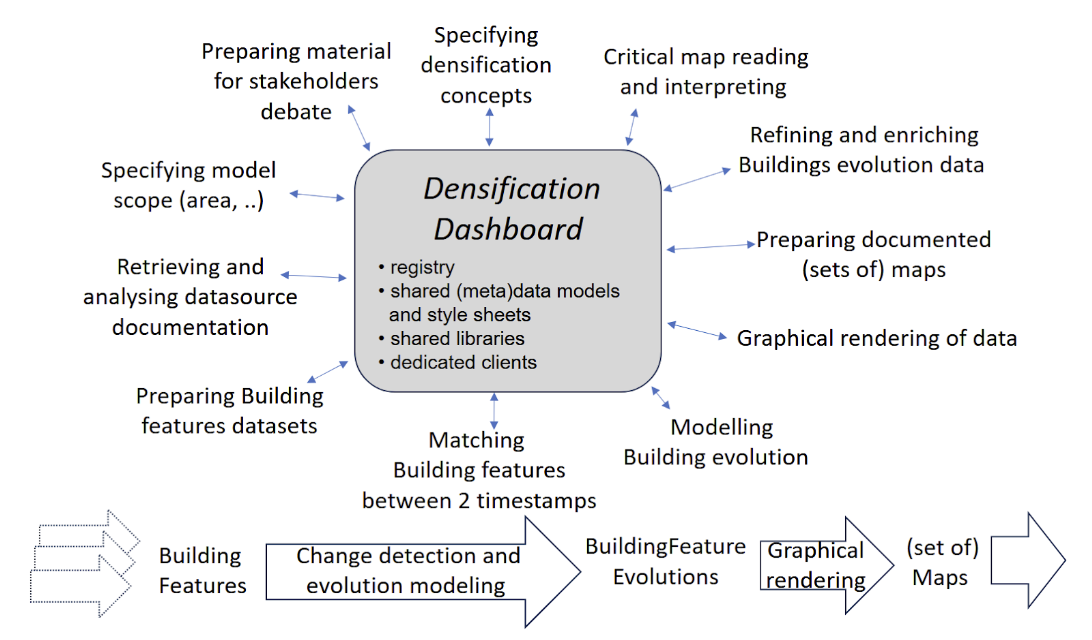
\includegraphics[width=0.8\linewidth]{figures/dashboard.png}
\caption{Components and usages of the co-operative dashboard. An example of a workflow within the dashboard, from building data to thematic maps is also detailed.}
\label{fig:dashboard} 
\end{figure*}

The core components of the dashboard are: (i) a registry for concepts, maps,  datasources, datasets, processes ; (ii) shared models for describing these items  ; (iii) shared libraries and software for computing building evolution and producing maps ; (iv) different clients to interact with the previous components (including a web application displaying maps, which corresponds to the more classical view of a ``dashboard'').

% Data and software availability
\subsection{Implementation}

%\vspace{-0.5cm}

Our dashboard implementation aims for genericity, reproducibility, and minimisation of deployment constraints. Therefore, the \texttt{git} software was chosen, ensuring also full transparency and tractability of the process. The dashboard itself is a git repository available at \url{https://github.com/subdense/dashboard}.

The repository includes different registry files, as plain text markdown files, which list and provide unique identifiers for objects. These include registries for concepts, maps, datasources, datasets, and processes. Comments and feedback on objects are also stored in these files.

At this stage, three types of clients are proposed to interact with the dashboard: (i) the git client itself, by directly committing changes to the repository; (ii) a website, deployed automatically through github pages at \url{https://subdense.github.io/dashboard/}, for which user feedback is collected using a Javascript git library (currently under implementation); (iii) the open software QGIS for processing data, map reading and enrichment (python plugins for QGIS which run processes from the dashboard are also currently being implemented, and map style sheets are provided).


\subsection{Building change detection and Geospatial User Feedback}

%\vspace{-0.5cm}

Processes in the dashboard include step-by-step descriptions of how a user retrieved data, processed it, produce maps, etc., but furthermore automated processes to run algorithms analysing data. One key process is change detection in building data, for which we use vector data matching algorithms \citep{olteanu2015knowledge}. Building features between two dates are matched using the Geometric Matching of Areas algorithm \citep{harvey1998geometric}, are then automatically interpreted as changes following a \texttt{BuildingFeatureEvolution} model following \cite{claramunt1997qualitative}, and finally filtered to distinguish specific cases of evolutions due to changes in data sources (for example, for France IGN BDTOPO changed between 2011 and 2021 the minimum threshold to include buildings and the way to compute building boundaries).

\begin{figure*}[ht]
  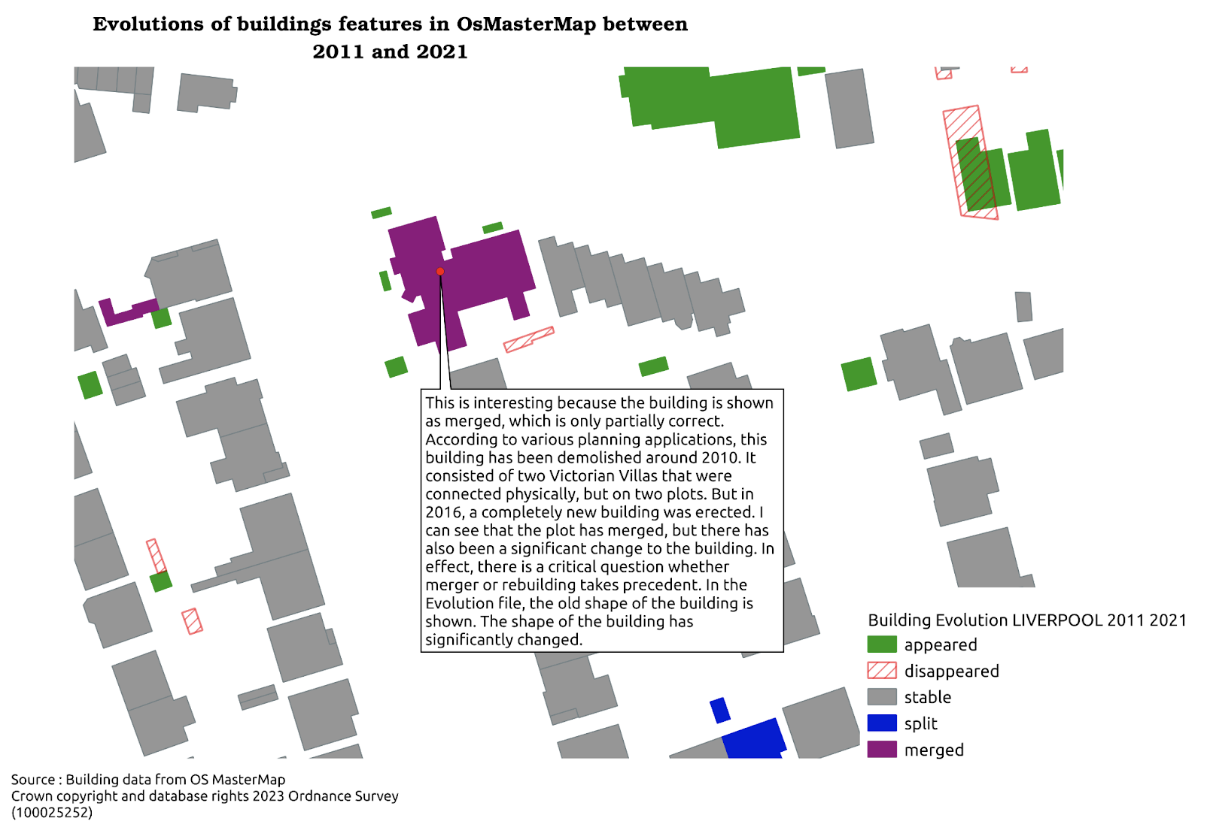
\includegraphics[width=0.8\linewidth]{figures/guf.png}
\caption{Example of Geospatial User Feedback on the building evolution model, with change detection on OSMasterMap 2011 and 2021 data for Liverpool.}
\label{fig:guf} 
\end{figure*}

Maps are then produced using QGIS, and experts can provide Geospatial User Feedback (GUF) \citep{zabala2021geospatial}, either to rework the data model, to refine the automatic interpretation process, or more generally to gain knowledge on data quality or the process itself. Such an example of GUF is shown in fig.~\ref{fig:guf}, with the example of a specific area in Liverpool for which a local spatial planning expert went on the field and checked planning documents, to invalidate a building evolution produced by the algorithm. This feedback will then be used to reconsider the algorithm parametrisation or its internal mechanisms.


\subsection{Data and software availability}

Software, metadata, data, maps, and results produced in this project are openly available on the git dashboard repository. Building data is available under an Open Licence for France (compatible with CC-By) from the data product BD TOPO, while for the UK and Germany, data can be accessed and used freely for research purposes after signing agreements with local mapping agencies. Our data on building evolution derived from these will be made available under the same terms. We plan to also compute building evolution data for UK and Germany using OpenStreetMap (for years having sufficient coverage), to ensure that produced evolution dataset are available under an Open Licence for all countries.




\conclusions[Perspectives]

Future work include the definition of quality control methods to document quality criteria for the building evolution data, and the extraction of a knowledge graph based on the different metadata fragments to depict the dashboard content and automate some tasks like generation of web pages with relevant quality information aside maps: scope, provenance, usage.    

We also plan to enrich the process with evolutions of other features and to engage with local stakeholders to clarify the evolutions concepts.

\begin{acknowledgements}
This research was performed during the project SUBDENSE funded by the seventh Open Research Area in social sciences (ANR, DFG, ESRC ES/X008290/1).
\end{acknowledgements}


%% REFERENCES

%% The reference list is compiled as follows:

%\begin{thebibliography}{}

%\bibitem[AUTHOR(YEAR)]{LABEL1}
%REFERENCE 1

%\bibitem[AUTHOR(YEAR)]{LABEL2}
%REFERENCE 2

%\end{thebibliography}

%% Since the AGILE LaTeX package includes the BibTeX style file agile.bst, authors experienced with BibTeX only have to include the following two lines:
%%

\bibliographystyle{copernicus-agile}
\bibliography{biblio.bib}

%%
%% URLs and DOIs can be entered in your BibTeX file as:
%%
%% URL = {http://www.xyz.org/~jones/idx_g.htm}
%% DOI = {10.5194/xyz}


%% LITERATURE CITATIONS
%%
%% command                        & example result
%% \citet{jones90}|               & Jones et al. (1990)
%% \citep{jones90}|               & (Jones et al., 1990)
%% \citep{jones90,jones93}|       & (Jones et al., 1990, 1993)
%% \citep[p.~32]{jones90}|        & (Jones et al., 1990, p.~32)
%% \citep[e.g.,][]{jones90}|      & (e.g., Jones et al., 1990)
%% \citep[e.g.,][p.~32]{jones90}| & (e.g., Jones et al., 1990, p.~32)
%% \citeauthor{jones90}|          & Jones et al.
%% \citeyear{jones90}|            & 1990



%% FIGURES

%% When figures and tables are placed at the end of the MS (article in one-column style), please add \clearpage
%% between bibliography and first table and/or figure as well as between each table and/or figure.

% The figure files should be labelled correctly with Arabic numerals (e.g. fig01.jpg, fig02.png).


%% ONE-COLUMN FIGURES

%%f
%\begin{figure}[t]
%\includegraphics[width=8.3cm]{FILE NAME}
%\caption{TEXT}
%\end{figure}
%
%%% TWO-COLUMN FIGURES
%
%%f
%\begin{figure*}[t]
%\includegraphics[width=12cm]{FILE NAME}
%\caption{TEXT}
%\end{figure*}
%
%
%%% TABLES
%%%
%%% The different columns must be seperated with a & command and should
%%% end with \\ to identify the column brake.
%
%%% ONE-COLUMN TABLE
%
%%t
%\begin{table}[t]
%\caption{TEXT}
%\begin{tabular}{column = lcr}
%\tophline
%
%\middlehline
%
%\bottomhline
%\end{tabular}
%\belowtable{} % Table Footnotes
%\end{table}
%
%%% TWO-COLUMN TABLE
%
%%t
%\begin{table*}[t]
%\caption{TEXT}
%\begin{tabular}{column = lcr}
%\tophline
%
%\middlehline
%
%\bottomhline
%\end{tabular}
%\belowtable{} % Table Footnotes
%\end{table*}
%
%%% LANDSCAPE TABLE
%
%%t
%\begin{sidewaystable*}[t]
%\caption{TEXT}
%\begin{tabular}{column = lcr}
%\tophline
%
%\middlehline
%
%\bottomhline
%\end{tabular}
%\belowtable{} % Table Footnotes
%\end{sidewaystable*}
%
%
%%% MATHEMATICAL EXPRESSIONS
%
%%% All papers typeset by Copernicus Publications follow the math typesetting regulations
%%% given by the IUPAC Green Book (IUPAC: Quantities, Units and Symbols in Physical Chemistry,
%%% 2nd Edn., Blackwell Science, available at: http://old.iupac.org/publications/books/gbook/green_book_2ed.pdf, 1993).
%%%
%%% Physical quantities/variables are typeset in italic font (t for time, T for Temperature)
%%% Indices which are not defined are typeset in italic font (x, y, z, a, b, c)
%%% Items/objects which are defined are typeset in roman font (Car A, Car B)
%%% Descriptions/specifications which are defined by itself are typeset in roman font (abs, rel, ref, tot, net, ice)
%%% Abbreviations from 2 letters are typeset in roman font (RH, LAI)
%%% Vectors are identified in bold italic font using \vec{x}
%%% Matrices are identified in bold roman font
%%% Multiplication signs are typeset using the LaTeX commands \times (for vector products, grids, and exponential notations) or \cdot
%%% The character * should not be applied as mutliplication sign
%
%
%%% EQUATIONS
%
%%% Single-row equation
%
%\begin{equation}
%
%\end{equation}
%
%%% Multiline equation
%
%\begin{align}
%& 3 + 5 = 8\\
%& 3 + 5 = 8\\
%& 3 + 5 = 8
%\end{align}
%
%
%%% MATRICES
%
%\begin{matrix}
%x & y & z\\
%x & y & z\\
%x & y & z\\
%\end{matrix}
%
%
%%% ALGORITHM
%
%\begin{algorithm}
%\caption{...}
%\label{a1}
%\begin{algorithmic}
%...
%\end{algorithmic}
%\end{algorithm}
%
%
%%% CHEMICAL FORMULAS AND REACTIONS
%
%%% For formulas embedded in the text, please use \chem{}
%
%%% The reaction environment creates labels including the letter R, i.e. (R1), (R2), etc.
%
%\begin{reaction}
%%% \rightarrow should be used for normal (one-way) chemical reactions
%%% \rightleftharpoons should be used for equilibria
%%% \leftrightarrow should be used for resonance structures
%\end{reaction}
%
%
%%% PHYSICAL UNITS
%%%
%%% Please use \unit{} and apply the exponential notation

%\copyrightstatement{TEXT} %% This section is optional and can be used for copyright transfers.

%\texlicencestatement Licence TEST


\end{document}




% For two-column wide figures use
\begin{figure*}[ht]
% Use the relevant command to insert your figure file.
% For example, with the graphicx package use
  \includegraphics[width=16cm]{figures/example_figure-2.png}
% figure caption is below the figure
\caption{An example figure spanning over both columns.}
\label{fig:1}       % Give a unique label
\end{figure*}
%




% For one-column wide figures use
\begin{figure}[ht]
% Use the relevant command to insert your figure file.
% For example, with the graphicx package use
  \includegraphics[width=8.2cm]{figures/agile-logo_cmyk.pdf}
% figure caption is below the figure
\caption{The logo of AGILE -- the Association of Geographic Information Laboratories in Europe.}
\label{fig:2}       % Give a unique label
\end{figure}
%

